\documentclass[a4paper]{article}
\usepackage[dutch]{babel}
\usepackage[utf8x]{inputenc}
\usepackage{amsmath,graphicx,hyperref,parskip,setspace,fancyhdr,changepage}
\usepackage[margin=1in]{geometry}
\usepackage[colorinlistoftodos]{todonotes}

\setlength{\parindent}{0mm}
\linespread{1.4}

\newcommand{\rcom}[1]{\textbf{\textcolor{red}{#1}}}
\newcommand{\com}[2]{\texttt{#1}\mbox{}\vspace{-2ex}\begin{adjustwidth}{0.8cm}{} #2 \end{adjustwidth}}
\newcommand{\ttt}[1]{\texttt{#1}}

\pagestyle{fancy}

\title{Symbolische manipulatie}
\author{Rik~Voorhaar~(3888169) - Jan-Willem~van~Ittersum~(3992942) - Jurre~Corver~(3905985)\\
Begeleider: Joost Houben}

\begin{document}
\maketitle
\clearpage

%\begin{abstract}
%Your abstract.
%\end{abstract}

\section{Introductie}
In deze opdracht hebben we een eigen computeralgebrasysteem (CAS) ontwikkeld om symbolisch te kunnen rekenen zoals dat bijvoorbeeld in Mathematica gebeurt. Wiskundige formules worden hiervoor opgeslagen in een zogenaamde expressie-boom. Behalve dat deze representatie kan worden gebruikt om berekeningen te doen, is deze geschikt voor symbolische manipulaties, zoals optellen, vermenigvuldigen, maar ook differenti\"eren en oplossen van sommige polynoom~vergelijkingen. De code behordende bij dit project kan gevonden worden op \url{https://github.com/JurreCorver/SymbolischeManipulatie}.


\section{Theorie}
%Beschrijving van de theorie
Een expressie-boom is een samenhangende, gerichte graaf, waarbij elke knoop (op \'e\'en knoop na) exact \'e\'en inkomende zijde heeft en een willekeurig aantal uitgaande zijden. De unieke knoop zonder inkomende zijde noemen we \textit{de wortel}, een knoop met minstens \'e\'en uitgaande zijde noemen we \textit{een interne knoop} en een knoop zonder uitgaande zijde noemen we \textit{een blad}. In de knopen van deze expressie-boom wordt een berekening opgeslagen. Een blad is een constante of een variabele, bijvoorbeeld $3$ of $x$. Een interne knoop (de wortel is ook een interne knoop) is een operator of een functie. Naast de binaire operatoren optellen $+$, aftrekken $-$, vermenigvuldigen $*$, delen $/$, modulo $\%$ en machtsverheffing $**$ die gekenmerkt worden door het feit dat er zowel links als rechts van de operator \'e\'en argument nodig is, is er een negatie operator $-$ die alleen een argument rechts heeft. Vergelijk bijvoorbeeld de binaire operator $-$ in $5-x$ met de negatie operator $-$ in $-x+2$. Een voorbeeld van een expressieboom zie je in \ref{fig:boom}.

\begin{figure}[!htb]
	\centering
	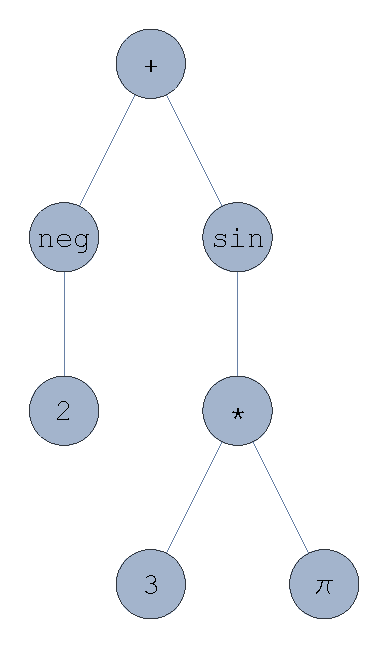
\includegraphics[width=0.25\textwidth]{expressionTree}
	\caption{Voorbeeld van een expressieboom. In infix notatie  kan de expressie weergegeven in deze boom gegeven worden door $-2+\sin(3\times \pi)$. In postfix notatie is het $3\,\pi\times\sin 2\, \mathrm{neg}\,+$.}\label{fig:boom}
\end{figure}

\rcom{Iets over infix (normale wiskunde) versus postfix (RPN) notatie. Shunting-yard doet infix->postfix->boom.}

\section{Algoritmen}
%Beschrijving van de gebruikte algoritmen, denk hierbij ook aan bijvoorbeeld de complexiteit en de gebruikte datastructuren
\subsection{Shunting-yardalgoritme}
Een gebruiker vindt infix notatie het makkelijkst te gebruiken, en zal graag zijn invoer dus ook in infix notatie aan een programma willen doorvoeren. De meest nuttige manier om een expressie op te slaan en te bewerken blijkt echter in de vorm van een expressieboom te zijn. Het Shunting-yardalgoritme maakt de vertaalslag van de infix notatie van de gebruiker naar postfix notatie, en de vertaling van postfix notatie naar een expressieboom is vrij gemakkelijk. Het algoritme is gepubliceerd door Dijkstra in 1961. 

We gaan niet het algoritme in volledig detail beschrijven, we behandelen het slechts in grove lijnen aan de hand van voorbeelden. We beginnen met een string met een expressie in infix notatie, bijvoorbeeld \texttt{`2-3*3'}. Dit splitsen we dan op in kleine stukken genaamd `tokens'. In dit geval: \texttt{`2',`-',`3',`*'}. 

Dan maken we vervolgens twee lijsten aan, de \ttt{stack} en de \ttt{output}. We gaan dan van links naar rechts door de lijst van tokens heen en volgen de volgende procedure uit:
\begin{enumerate}
\item Indien de token een getal is, stop hem in de \ttt{output}.
\item Als de token een comma is, verplaats dan steeds het bovenste element van de \ttt{stack} naar de \ttt{output} totdat het laatste element van de \ttt{stack} een \ttt{`('} is.
\item Als de token een binaire operator (\ttt{-,+,*,/,\%,**}) is,  blijf dan aan de hand van de precedentie operatoren van de \ttt{stack} naar de \ttt{output} verplaatsen totdat het laatste element van de \ttt{stack} geen operator meer is. De \ttt- token wordt dan op een speciale manier behandeld, omdat het zowel negatie als aftrekken kan betekenen.
\item Als de token \ttt{`('} is, kijk dan of het laatste element op de \ttt{output} een functie is. Zo ja, verplaats dan de functie naar de \ttt{stack}. Stop het haakje op de \ttt{output}.
\item Als de token \ttt{`)'} is, verplaats dan elementen van de \ttt{stack} naar de \ttt{output} totdat er een \ttt{'('} wordt tegengekomen. Verwijder dan de \ttt{'('} van de \ttt{stack}. Indien de bovenkant van de \ttt{stack} nu een functie is, voeg hem dan toe aan de output.
\item Als de token een bekende variabele (e.g. \ttt{`pi'}) is, voeg zijn waarden dan toe aan de \ttt{output}.
\item Als de token in geen van de bovenstaande gevallen zit, voeg hem dan als onbekende variabele toe aan de \ttt{output}.
\item Als we door de lijst van tokens heen zijn, voeg dan alle elementen van de \ttt{stack} toe aan de \ttt{output}.
\end{enumerate}

Deze procedure geeft dan een uitdrukking in postfix notatie terug. Met het volgende alrogritme word dan de postfix notatie naar een expressieboom veranderd. We itereren de volgende procedure over de \ttt{output} heen, en noemen de elementen van \ttt{output} weer tokens. We hebben om te beginnen eerst weer een lege \ttt{stack}.
\begin{enumerate}
\item Als de token een functie is, haal dan $n$ elementen van de \ttt{stack} af, waar $n$ de hoeveelheid argumenten is die de functie aanneemt. Voeg vervolgens de functie als knoop toe de \ttt{stack} met als kinderen de $n$ argumenten. 
\item Als de token een binaire operator is, voeg de operator als knoop toe aan de \ttt{stack} met als kinderen de twee operanden.
\item Als de token geen functie of operator is, voeg hem dan aan de \ttt{stack} toe.
\end{enumerate}
Na deze procedure hebben we bij invoer van geldige syntax slechts \'e\'en element over in de \ttt{stack}. Dit element is dan de expressieboom met als bovenste knoop de wortel van de boom. Het gehele algoritme om infix notatie om te zetten in postfix notatie en vervolgens in een expressieboom is van orde $\mathcal{O}(n)$, aangezien er precies \'e\'en keer over de lijst van tokens word ge\"itereerd, en ook precies \'e\'en keer over de \ttt{output} wordt ge\"itereerd (en de output is vervolgens maximaal even lang als de lijst van tokens).

\subsection{Simplify algoritme}
Voor vele andere functies in het programma is het erg nuttig om symbolische vergelijkingen te kunnen versimpelen. Denk hier bijvoorbeeld aan expressies als \ttt{x-x} naar \ttt{0} te versimpelen. Daarom is de functie \ttt{simplify(expression)} ge\"implementeerd die de expressie \ttt{expression} zoveel mogelijk probeert te versimpelen. We zullen hier een summiere omschrijving geven over de werking van deze functie. De \ttt{simplify} functie roept de \ttt{simplifyStep} functie net zo vaak, met een maximum van 20 keer, aan tot dat de uitdrukking niet meer veranderd na verdere toepassing van \ttt{simplifyStep}. De \ttt{simplifyStep} functie gebruikt standaard rekenregels voor r\"eele getallen om polynomiale uitdrukkingen zo ver mogelijk te versimpelen. Bij functies versimpeld de functie enkel de argumenten. Verder heeft \ttt{simplify} een optioneel argument die bepaald of bij elke toepassing van \ttt{simplifyStep} de expressie wordt ge\"expandeerd. 

\subsection{Grafische omgeving}
De grafische omgeving maakt gebruik van  \ttt{tk} voor de weergave. Deze interpreteert dan de invoer van de gebruiker en voert deze uit door \ttt{expression\_template.py} in te laden. De gebruiker heeft dan de optie om de uitvoer weer te geven met \LaTeX. Dit werkt door de expressie om te vormen tot \LaTeX code. Deze \LaTeX code wordt vervolgens naar een \ttt{.tex} bestand geschreven en uitgevoerd door \ttt{latex} aan te roepen, wat dan weer een \ttt{.dvi} bestand als uitvoer geeft. Dit \ttt{.dvi} bestand wordt dan met behulp van \textit{GhostScript} omgevormd naar een \ttt{.png} bestand die wordt weergegeven door \ttt{tk}.


\subsection{solvePolynomial algoritme}
Het solvePolynomial algoritme neemt een polynomiale vergelijking en een variabele als argument en probeert dan een oplossing te vinden via de volgende stappen.
\begin{enumerate}
\item Test of er wel een vergelijking is ingevoerd. Als dit zo is, haal dan de rechterkant van de vergelijking naar de linkerkant via gewoonlijke algebra. Is dit niet het geval neem dan aan dat de wortel van de vergelijking wordt bedoeld.
\item Sla de polynoom op als een lijst met co\"effici\"enten. 
\item Controleer wat de kleinste macht in de vergelijking is. Als deze kleiner is dan 0, vermenigvuldig dan met deze macht. Is hij groter dan 0, deel door deze macht. Voeg in het tweede geval 0 toe als oplossing van de vergelijking.
\item Controleer nu de graad van de vergelijking. Is de graad 0, dan bestaat er geen oplossing. Is de graad 1, 2 of 3 geef dan de oplossing gebruikmakend van bekende algoritmes. In andere gevallen is er geen oplossing.
\item Return de oplossing
\end{enumerate}

\section{Documentatie}
%Documentatie over het gebruik van de code
\subsection{Installatie}
Om dit programma te gebruiken zijn naast een werkende Python 3.4 distributie enkele Python packages nodig. De niet-standaard packages zijn: \texttt{numpy, pillow, scipy, tkinter}.
Verder heeft de grafische gebruikers omgeving onderstuining voor het weergeven van de output met behulp van \LaTeX. Hiervoor is dus een werkende \LaTeX~distributie vereist. Daarbij is het ook benodigd om \emph{GhostScript} geinstalleerd te hebben. Voor \emph{Windows} gebruikers is het verder specifiek vereist om de 32-bit versie van \emph{GhostScript} te gebruiken en het pad naar \texttt{gswin32c.exe} toe te voegen aan de \texttt{\%path\%} systeemvariabele.

\subsection{Grafische omgeving}
De grafische omgeving kan gebruikt worden door \texttt{tkmain.pyw} uit te voeren. Dit kan ook vanuit de command-line door \texttt{python tkmain.pyw} uit te voeren.  De verschillende componenten van de omgeving zullen worden uitgelegd met referentie naar figuur \ref{fig:screenshot}

\begin{figure}[!htb]
  \centering
  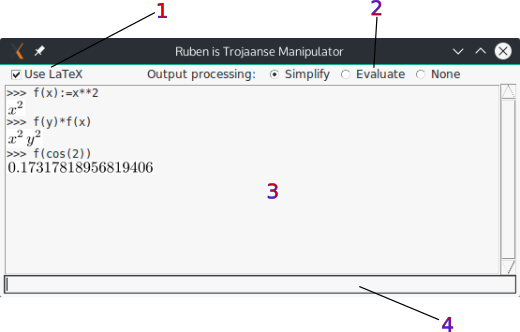
\includegraphics[width=0.6\textwidth]{screenshot.png}
  \caption{Screenshot van de grafische omgeving}
  \label{fig:screenshot}
\end{figure}

\begin{enumerate}
\item Met de \texttt{Use LaTeX} wordt gespecificeerd of de output door \LaTeX wordt verwerkt voor dat deze wordt weergegeven. Indien deze optie niet geselecteerd is zal de output als plain-text worden weergegeven.
\item De \texttt{Output processing} optie specificeerd hoe de input wordt verwerkt. Indien \texttt{Simplify} is aangevinkt zal de expressie zo veel mogelijk versimpeld worden. Terwijl bij het aanvinken van \texttt{Evaluate} de expressie wordt uitgerekend indien deze numeriek is, en anders onversimpeld wordt weergegeven. Als laatste zorgt de \texttt{None} optie juist dat de expressie niet wordt berekend en direct wordt weergegeven.
\item Dit is het scherm waar de output wordt weergegeven. Hier wordt de input van de gebruiker met \texttt{>>>} er voor weergegeven, en telkens op de regel daarna de output bij de regel input erboven. Indien er fouten optraden tijdens het uitvoeren van de input wordt dit hier ook weergegeven.
\item In dit scherm kan de gebruiker zijn input invoeren. Als de gebruiker de \texttt{Enter} toets indrukt wordt de input ge\"evaluaeerd. De pijltjestoetsen naar boven en onder kunnen worden gebruikt om de vorige input nog een keer te gebruiken.
\end{enumerate}

\subsection{Syntax}
De invoer ondersteund standaard operaties op getallen die met symbolen \texttt{*, +, -, **, /, \%} kunnen worden ingevoerd. Verder kunnen ronde haaken \texttt{( )} worden gebruikt. Enkele voorbeelden:
\begin{adjustwidth}{1.5cm}{}
\setstretch{0.9}
\texttt{>>> 2+2-1}\\
$1$\\
\texttt{>>> (2**3)/2}\\
$4$\\
\texttt{>>> 7 \% 3}\\
$1$
\end{adjustwidth}
Ook zijn standaard functies als \texttt{sin, ln, gamma, gcd} ge\"implementeerd. %De specifieke details over deze functies zijn te vinden in de volgende sectie. 
De lijst met alle ge\"implementeerde functies is te vinden in de volgende sectie. Er is verder ook ondersteuning voor complexe getallen. De imaginaire constante wordt aangeduid met \texttt{i}. Andere standaard constanten zijn \texttt{pi, e, phi}. Voorbeeld:
\begin{adjustwidth}{1.5cm}{}
\setstretch{0.9}
\texttt{>>> i**2}\\
$-1$\\
\texttt{>>> exp(i*pi)-1}\\
$0$
\end{adjustwidth}
Naast standaard operaties is het ook mogelijk om zelf functies en constanten toe te voegen. Hiervoor kan \texttt{:=} gebruikt worden. Als links van de \texttt{:=} alleen een symbool staat, dan wordt wat rechts van de \texttt{:=} staat opgeslagen onder naam van het symbool aan de linkerkant. We kunnen bijvoorbeeld het volgende doen:
\begin{adjustwidth}{1.5cm}{}
\setstretch{0.9}
\texttt{>>> x:=5}\\
$5$\\
\texttt{>>> x**2}\\
$25$
\end{adjustwidth}
Functies kunnen op een vergelijkbare manier worden toegevoegd. Neem als voorbeeld:
\begin{adjustwidth}{1.5cm}{}
\setstretch{1}
\texttt{>>> f(x,y):=sin(x)*cos(y)}\\
$\mathrm{sin}(x)\,\mathrm{cos}(y)$\\
\texttt{>>> f(pi/2,pi)}\\
$-1$
\end{adjustwidth}
Als laatste is er ondersteuning voor een gelijkheids operator met \texttt{==} als symbool. Deze kan bijvoorbeeld worden gebruikt bij invoeren van vergelijkingen.


\subsection{Lijst van commando's}
\rcom{na afloop op alfabetische volgorde zetten\\}
\com{exit()}{Sluit het programma af.}
\com{d(f(x),x)}{Berekent de afgeleide van \texttt{f(x)} naar de variabele \texttt{x}. Indien de afgeleide van de functie niet bekend is wordt een foutmelding gegeven. Voorbeeld:\vspace{-0.5ex}}
\begin{adjustwidth}{1.5cm}{}
\setstretch{1}
\texttt{>>> d(sin(x)+2,x)}\\
$\cos(x)$
\end{adjustwidth}

\com{sin(x), arcsin(x), cos(x), arccos(x), tan(x), arctan(x), ln(x), exp(x), floor(x), gamma(x)}{Geeft de bijbehorende standaardfunctie als functie van \texttt{x}.}
%\com{sin(x)}{Geeft de sinus van \texttt{x}.}
%\com{arcsin(x)}{Geeft de arcsinus van \texttt{x}.}
%\com{cos(x)}{Geeft de cosinus van \texttt{x}.}
%\com{arccos(x)}{Geeft de arccosinus van \texttt{x}.}
%\com{tan(x)}{Geeft de tangus van \texttt{x}.}
%\com{arctan(x)}{Geeft de arctangus van \texttt{x}.}
%\com{log(x,y)}{Geeft het logaritme van \texttt{x} in basis \texttt{y}. Equivalent aan \texttt{ln(x)/ln(y)}.}
%\com{ln(x)}{Geeft het natuurlijk logaritme van \texttt{x}.}
%\com{exp(x)}{Geeft het exponent van \texttt{x}.}
%\com{floor(x)}{Neemt de floor van \texttt{x}.}
%\com{gamma(x)}{Geeft de gamma functie van \texttt{x}.}
\com{log(x,y)}{Geeft het logaritme van \texttt{x} in basis \texttt{y}. Equivalent aan \texttt{ln(x)/ln(y)}.}
\com{polygamma(x,y)}{Geeft de \texttt{y}'de orde polygamma functie van \texttt{x}.}

\rcom{misschien ook nog even round en ceil toevoegen voor compleetheid?}

\rcom{nog toevoegen:\\}
\com{solvePolynomial(eq, var)}{Geeft de oplossing van een polynomiale vergelijking in de variabele \textit{var}. Bijvoorbeeld $x^{10} = 1024$ of $x^2 + 1/x = 10$}
\com{numIntegrate(expressie, x, l, r, numsteps)}{Numeriek bepalen van $\int_{\texttt{l}}^\texttt{r} \texttt{expressie} \; \mathrm{d}\texttt{x}$ door middel van een Riemann benadering in \texttt{numsteps} stappen.}
\com{gcd(n,m)}{Geeft de grootste gemene deler van twee gehele getallen \texttt{n} en \texttt{m}.}
\com{polQuotient(pol1, pol2, x)}{Geeft het quotient van de deling van \texttt{pol1} door \texttt{pol2} met rest, waarbij \texttt{pol1} en \texttt{pol2} polynomen in \texttt{x} zijn.}
\com{polRemainder(pol1, pol2, x)}{Geeft de rest van de deling van \texttt{pol1} door \texttt{pol2}, waarbij \texttt{pol1} en \texttt{pol2} polynomen in \texttt{x} zijn.}
\com{polIntQuotient(pol1, pol2, x)}{Geeft het quotient van de deling van het polynoom \texttt{pol1} door het polynoom \texttt{pol2} met rest over de gehele getallen, waarbij \texttt{pol1} en \texttt{pol2} polynomen met gehele co\"effici\"enten in \texttt{x} zijn.}
\com{polIntRemainder(pol1, pol2, x)}{Geeft de rest van de deling van \texttt{pol1} door \texttt{pol2} over de gehele getallen, waarbij \texttt{pol1} en \texttt{pol2} polynomen in \texttt{x} zijn.}
\com{polContent(pol,x)}{Geeft de content van het polynoom \texttt{pol} in \texttt{x}.}
\com{polGcd(pol1,pol2,x)}{Geeft de grootste gemene deler van twee polynomen \texttt{pol1} en \texttt{pol1} met gehele co\"effici\"enten in \texttt{x}.}
\com{deg(pol,x)}{Geeft de graad van \texttt{pol} als polynoom in \texttt{x}.}

\section{Taakverdeling}
In het verslag is de volgende taakverdeling gehanteerd:

\com{Jurre} {Outline van het verslag gemaakt, solvePolynomial aan het verslag toegevoegd, theorie over postfix notatie, schrijven stukje over taakverdeling}
\com{Rik} {Stukje theorie over Shunting-yard}




\begin{thebibliography}{99}

\bibitem{c1} Wikipedia - Shunting-yard algorithm:
\url{https://en.wikipedia.org/wiki/Shunting-yard_algorithm}. 
 - geraadpleegd op 28 juni 2015
 \bibitem{c2} Houben, Joost. Expressie-bomen en Symbolische Manipulatie: WISB256 – Programmeren in de Wiskunde.


\end{thebibliography}



\end{document}